\documentclass[12pt]{report}
\usepackage{tikz}
\begin{document}
%general formula: \draw[parameters] (x, y) <SHAPE TYPE> (parameters)
% here's a basic drawing with lines and simple shapes 
\begin{tikzpicture}
\draw (0,0) -- (4,0) -- (4,4) -- (0,4) -- (0,0);
\draw (1,-1) -- (5,-1) -- (5,3) -- (1,3) -- cycle;
%rectangles specify lower left and upper right 
\draw (0,0) rectangle (6,6);
\draw (0,0) parabola (4,4);
\end{tikzpicture}

\vspace{5em}
%more shapes 
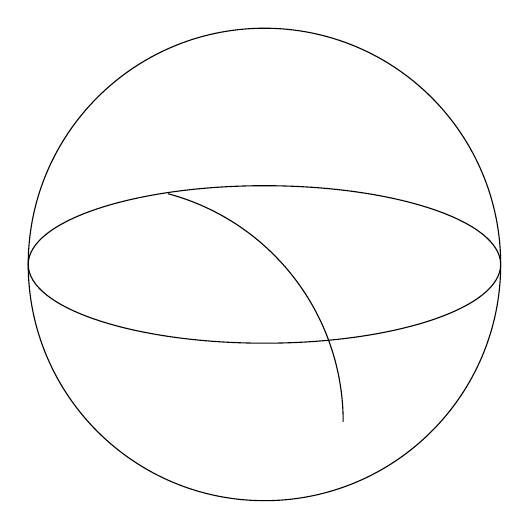
\begin{tikzpicture}
\draw (2,2) circle (3cm);
\draw (2,2) ellipse (3cm and 1cm);
\draw (3,0) arc (0:75:3cm);
\end{tikzpicture}

\vspace{5em}
%using parameters 
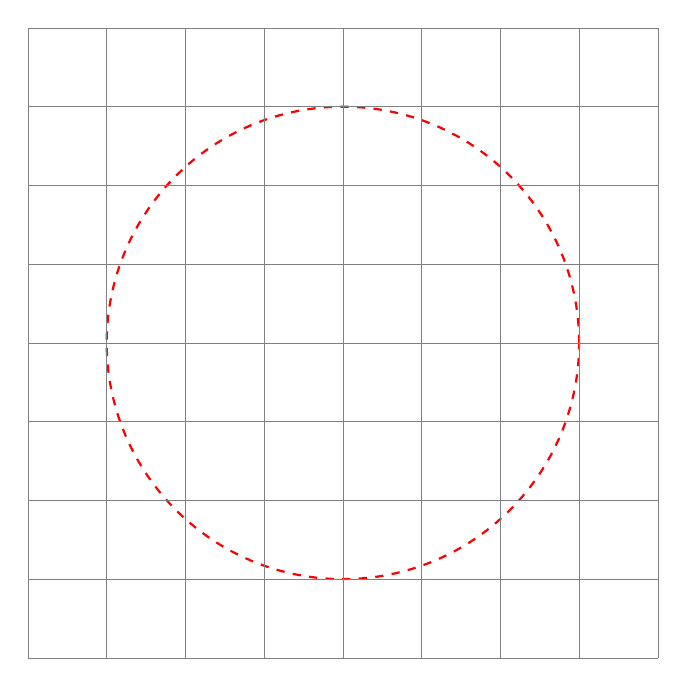
\begin{tikzpicture}
\draw[red,thick,dashed] (2,2) circle (3cm);
\draw[step=1cm,gray,very thin] (-2,-2) grid (6,6);
\end{tikzpicture}

\vspace{5em}
%using fill and shade commands

\begin{tikzpicture}
\fill[blue!40!white, draw=black] (0,0) rectangle (4,4);
\shade[left color=blue,right color=red] (5,0) rectangle (9,4);
\end{tikzpicture}



\vspace{5em}
%and now some arrows
\begin{tikzpicture}
\draw[thick,->] (0,0) -- (4.5,0);
\draw[thick,->] (0,0) -- (0,4.5);
\end{tikzpicture}

\vspace{5em}
%using nodes as anchors 
\begin{tikzpicture}
%the cardinal direction is where the text should be attached to the end
\draw[thick,->] node[anchor=north] {left node} (0,0) -- (4.5,0) node[anchor=south] {right node};
\draw[thick,->] (0,0) -- (0,4.5);
\end{tikzpicture}

\vspace{5em}
%for each loops
\begin{tikzpicture}
    \foreach \x in {0,1,2,3,4}
   \draw (\x cm,1pt) -- (\x cm,-1pt) node[anchor=north] {$\x$};
\end{tikzpicture}

%now. let's look at flow charts. This allows us to draw bayes networks with ease 
\tikzstyle{startstop} = [rectangle, rounded corners, minimum width=3cm, minimum height=1cm,text centered, draw=black, fill=red!30]
\tikzstyle{varr} = [circle,fill = white, draw=black]

% \begin{center}
% \begin{tikzpicture}
%     \node[shape=circle,draw=black] (B) at (0,0) {B};
%     \node[shape=circle,draw=black] (A) at (1.5,3) {A};
%     \node[shape=circle,draw=black] (C) at (3,0) {C};
%     \node[shape=circle,draw=black] (D) at (1.5, -3) {D};
%     \path [->] (B) edge node[left] {} (A);
%     \path [->](B) edge node[left] {} (C);
%     \path [->](D) edge node[left] {} (C);
% \end{tikzpicture}
% \end{center}
\vspace{5em}

%relative positioning
\begin{tikzpicture}[node distance=2cm] %how far apart by default
\node (start) [startstop] {Start};
\node (var) [varr, below of = start] {var};
\node (var2) [varr, right of = var] {var};
\node (var3) [varr, right of = var2] {var};
\node (start2) [startstop, below of = var] {end};
\draw [thick,->] (start) -- (var);
\end{tikzpicture}
\end{document}